\newpage

\section{Prediction Objective}

\quad One of the tasks for this project is the prediction of the number of sales of each one of the drinks (STELLA and BUD). To do that task there are two main modules that we can use, Univariate Analysis and Multivariate Analysis.\\

Univariate Analysis consiste in examening the relationship between a single column of data, that means that for this project we will create 2 univariate predictions, one for STELLA and the other for BUD. Also each one of those predictions will include multiple prediction methods, and the objective is to find the predictionmethod with the lowest error rate, for each of the drinks.

\begin{figure}[H]
    \centering
    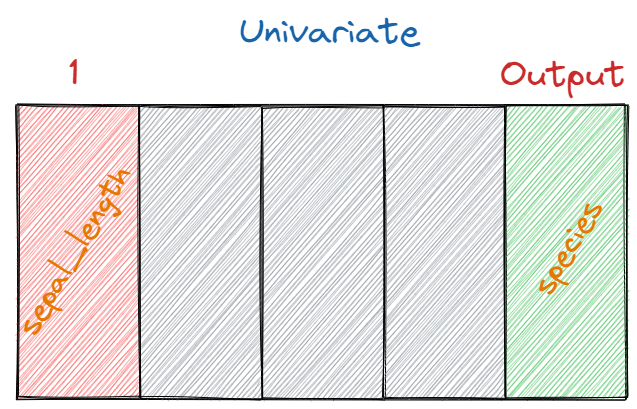
\includegraphics[width=0.4\textwidth]{assets/univariate_dataset.png}
    \caption{Univariate Analysis}
    \label{fig:univariate_dataset}
    \end{figure}

Multivariate Analysis is similar to the univariate analysis the main difference between the two is that multivariate analysis does not focus in only onde column of data, but instead use the data from multiple columns of data to predict. The data that will be included for the prediction of the sales of eac hdrink will include of course the sales of each respective drink, the precipitation and the maximum temperature on that day.


\begin{figure}[H]
    \centering
    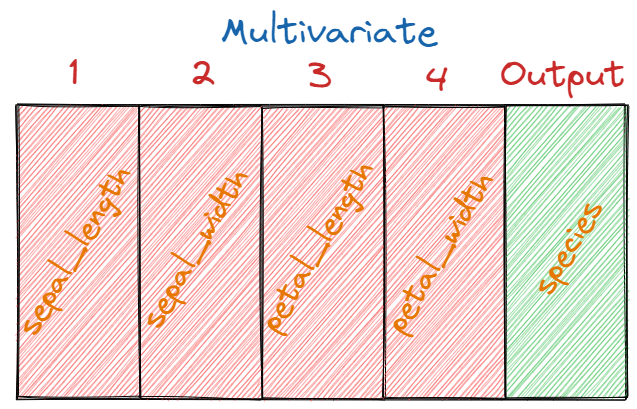
\includegraphics[width=0.4\textwidth]{assets/multivariate_dataset.png}
    \caption{Multivariate Analysis}
    \label{fig:mulivariate_dataset}
    \end{figure}


\newpage
\subsection{Univariate Analysis}

\quad For the Univariate Analysis there are multiple prediction methods that we will use, we will use mainly the machine learning amd forecast methods.\\

Our objective was to predict the last 20 weeks of each one of the drinks, for that we will use two methods for training the machine, they being the train-test split and the Growing and Rowling window split.\\

\subsubsection{Train-Test Split}

\quad In the Train-test split as we metion above, we will use Machine Learning prediction methods and Forecast prediction methods to predict the last 20 weeks of the sales. For each methods we create a script that run all of them and later will show the best methods. To determine the best method we will calculate the error rate from each method and of couse the method with the lowest error rate will be considerd the best prediction method.\\

For the Machine Learning prediction methods we will use the following:

\quad \textbullet "naive";

\quad \textbullet "ctree";

\quad \textbullet "cv.glmnet";

\quad \textbullet "kknn";

\quad \textbullet "mlp";

\quad \textbullet "randomForest";

\quad \textbullet "xgboost";

\quad \textbullet "cubist";

\quad \textbullet "lm";

\quad \textbullet "mars";

\quad \textbullet "pcr";

\quad \textbullet "plsr";

\quad \textbullet "cppls";

\quad \textbullet "rvm".\\

For the Forecast predictions methods we will sue the following:

\quad \textbullet "Holt-Winters";

\quad \textbullet "auto.arima";

\quad \textbullet "ets";

\quad \textbullet "nnetar".\\

After running the script that was developt by our group, we determine that the best prediction method was Holt Winters for the BUD drink, and mars for the STELLA drink, as they whete the methods with the lowest error rate from all the Machine Learning predictions methods and all the Forecast predictions methods. The next imagem will allows us to see the all the error rates from all the predictions methods.\\

\begin{figure}[H]
    \centering
    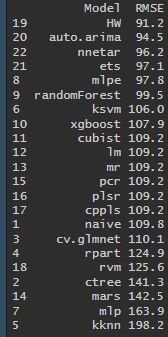
\includegraphics[width=0.4\textwidth]{assets/bud-split.jpeg}
    \caption{BUD - Machine Learning and Forecast Results}
    \label{fig:split_bud}
    \end{figure}

As we can see from this image, the best prediction method for the BUD drinks was Holt Winters, also the second best and the thir best methods were auto.arima and nmetar. Just a side note we can see that the best 3 methods come from Forecast predictions.\\

\begin{figure}[H]
    \centering
    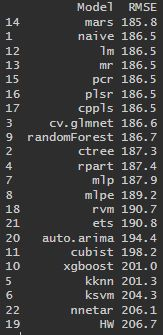
\includegraphics[width=0.4\textwidth]{assets/stella-split.jpeg}
    \caption{STELLA - Machine Learning and Forecast Results}
    \label{fig:split_stella}
    \end{figure}

As we can see from this image, the best prediction method for the STELLA drinks was mars, also the second best and the third best were naive and lm. Just a side note we can see that the best3 methods where form Machine Learning predictions.\\

For demonstration purposes here are the graphics of each of the predictions made by the best method for BUD and STELLA:

\begin{figure}[H]
    \centering
    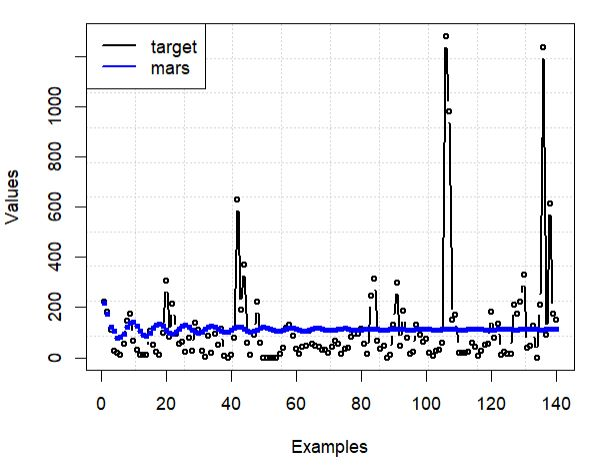
\includegraphics[width=0.7\textwidth]{assets/bud-split-graph.jpeg}
    \caption{BUD - Machine Learning and Forecast HW Graph}
    \label{fig:mulivariate_dataset}
    \end{figure}

\begin{figure}[H]
    \centering
    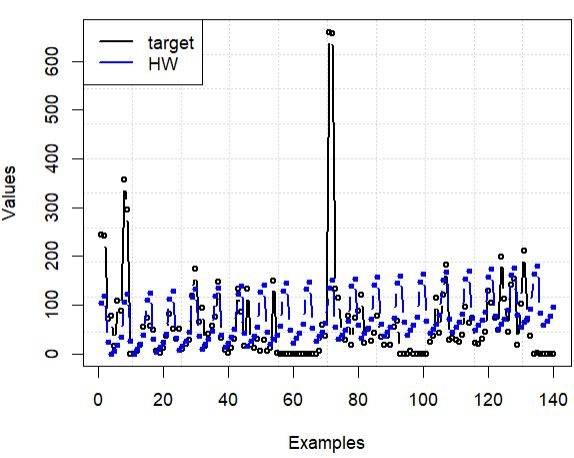
\includegraphics[width=0.7\textwidth]{assets/stella-split-graph.jpeg}
    \caption{STELLA - Machine Learning and Forecast mars Graph}
    \label{fig:mulivariate_dataset}
    \end{figure}


\newpage
\subsubsection{Growing and Rowling Window}

Similiar to above for this split we will use the same predictions methods, but we will also add the Weekly naive method.\\



\begin{figure}[H]
    \centering
    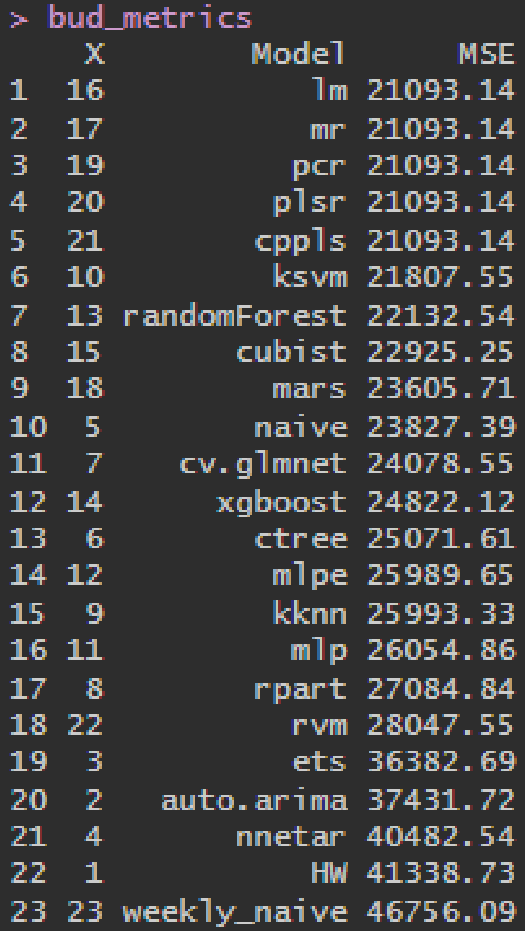
\includegraphics[width=0.4\textwidth]{assets/bud-gw.png}
    \caption{BUD - Growing and Rowling Window Results}
    \label{fig:gw_bud}
    \end{figure}

As we can see from this image, the best prediction method for the BUD drinks was lm, also the second best and the thir best methods were mr and pcr.\\

\begin{figure}[H]
    \centering
    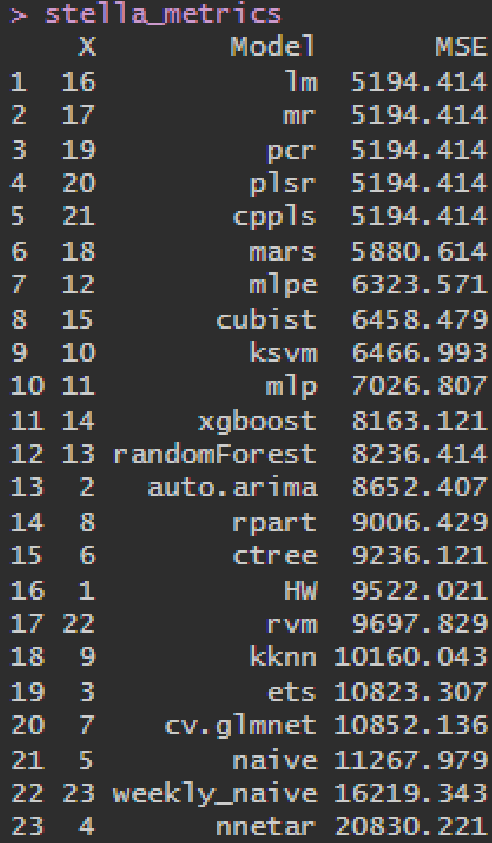
\includegraphics[width=0.4\textwidth]{assets/stella-gw.png}
    \caption{STELLA - Growing and Rowling Window Results}
    \label{fig:gw_stella}
    \end{figure}

As we can see from this image, the best prediction method for the STELLA drinks was lm, also the second best and the third best were mr and pcr.\\


For demonstration purposes here are the graphics of each of the predictions made by the best method for BUD and STELLA:


\begin{figure}[H]
    \centering
    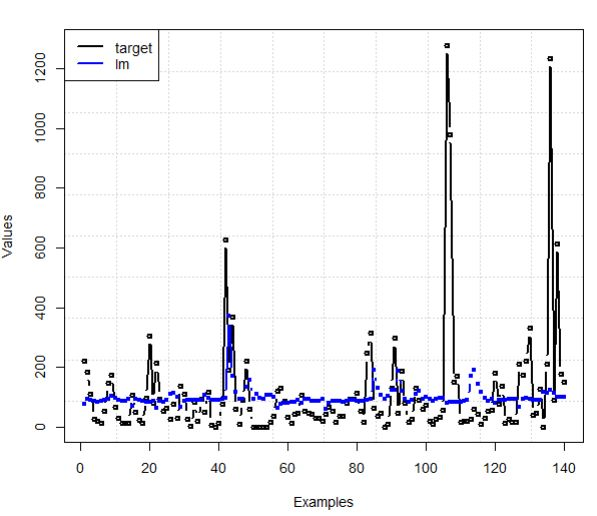
\includegraphics[width=0.65\textwidth]{assets/bud-GW.jpeg}
    \caption{BUD - Growing and Rowling Window lm Graph}
    \label{fig:gw_bud}
    \end{figure}


\begin{figure}[H]
    \centering
    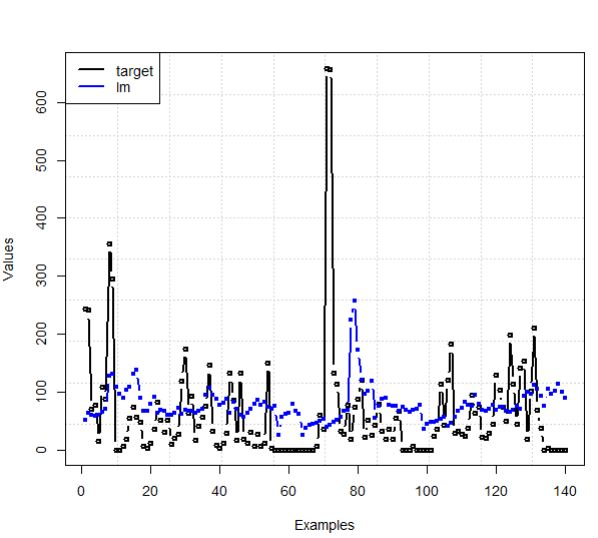
\includegraphics[width=0.65\textwidth]{assets/stella GW.jpeg}
    \caption{STELLA - Growing and Rowling Window lm Graph}
    \label{fig:gw_stella}
    \end{figure}
    
\newpage
\subsection{Multivariate Analysis}

\quad The Multivariate Analysis is similiar to the Univariate Analysis, the diference is that in this one we will use more than a set of data, in this project we will use the precipitation and the maximum temparature to assiste in the prediction of sales for each of the drinks.\\


For the Multivariate Analysis we create a neural network to assist in the prediction of sales for each of the drinks:

\begin{figure}[H]
    \centering
    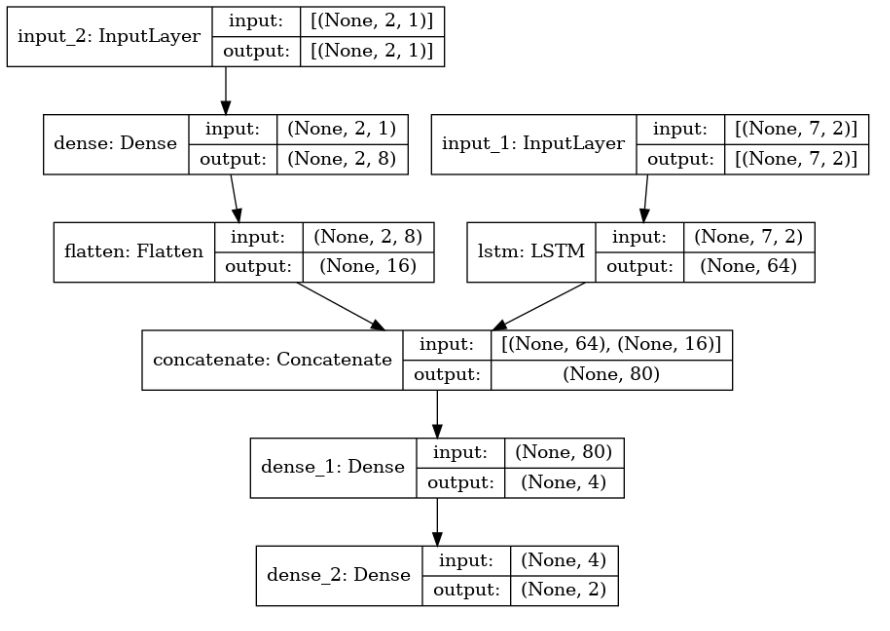
\includegraphics[width=0.8\textwidth]{assets/rede neuronal.jpeg}
    \caption{Neural Network}
    \label{fig:neural_network}
    \end{figure}


For the prediction we will use a split of Growing Window to predict the last 20 weeks of sales, for each drink, with a step of 7. The next image represents the results of the error mean of the 20 weeks prediction:\\


\begin{figure}[H]
    \centering
    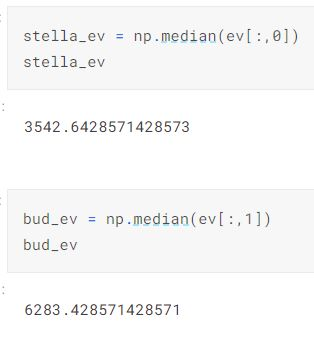
\includegraphics[width=0.4\textwidth]{assets/erros-previsao.jpeg}
    \caption{Mean of MSE Error for STELLA and BUD}
    \label{fig:notas}
    \end{figure}

For demonstration purposes here are the graphics of each of the predictions made for the BUD and STELLA:\\

\begin{figure}[H]
    \centering
    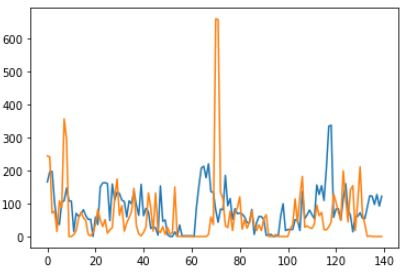
\includegraphics[width=0.6\textwidth]{assets/multi-stella.jpeg}
    \caption{STELLA - Multivariate Analysis Results}
    \label{fig:notas}
    \end{figure}

\begin{figure}[H]
    \centering
    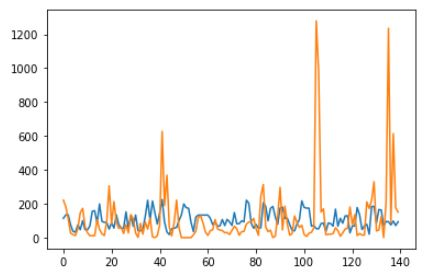
\includegraphics[width=0.6\textwidth]{assets/multi-bud.jpeg}
    \caption{STELLA - Multivariate Analysis Results}
    \label{fig:notas}
    \end{figure}







